\section{Design}

All building blocks in this thesis are developed with the purpose in mind to give the user the possibility to visualize and interact with complex 2D and 3D data, while being able to easily extend the library.
To enable this kind of functionality, a lot of parts of the infrastructure need to work seamlessly together.
Certain design choices had to be made to guarantee this. As speed is the most constraining factor, this chapter will start by introducing the design choices that had to be made in order to achieve state of the art speed.

\vspace{1em}
\begin{minipage}{\linewidth}
    \centering
    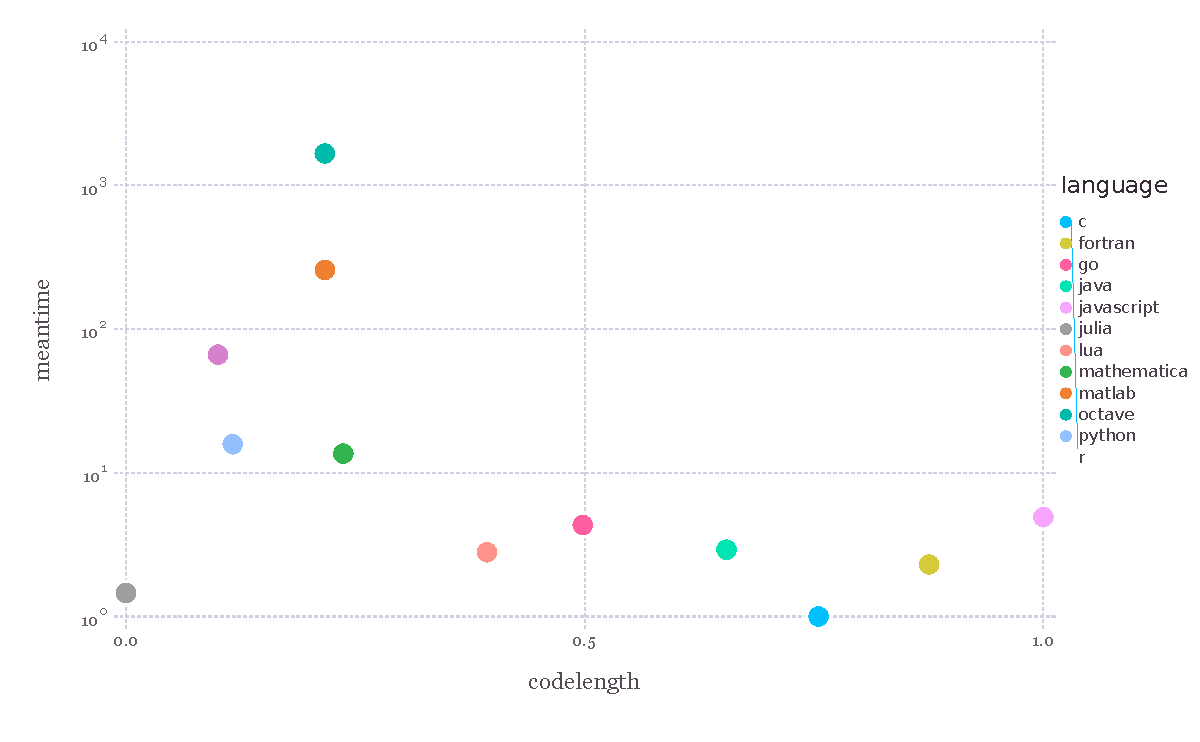
\includegraphics[width=0.9\linewidth]{graphics/julia_bench.pdf}
    \captionof{figure}[Volume Visualization]{Languages speed relative to C (averaged benchmark results), plotted against the length of the needed code (Source in Appendix)}
    \label{fig:juliabench}
\end{minipage}

\subsubsection{Speed}
Speed is mainly a usability factor. It's a factor, that can make a software unusable, or render it unproductive. Because of this, speed has taken a high priority in this thesis. As general coding productivity is also a concern, this thesis is set on using a high level language.
Historically, these two demands can't be both satisfied.
How to achieve state of the art speed with a high level language is an ongoing research and basically the holy grail of language design.
Luckily, there is a new programming language namely Julia building upon the compiler infrastructure \ac{LLVM}, promising a concise, high-level programming style, while approaching C-performance.
This is well illustrated in figure \ref{fig:juliabench}. Code length is an ambiguous measure for conciseness, but if the code is similarly refactored it is a good indicator of how many lines of code need to be written to achieve the same goal.
\ac{LLVM} is an impressive compiler infrastructure, which has front ends for different languages and back-ends for different chip architectures. 
A language designer has the task, to emit \ac{LLVM} \ac{IR}, which than gets just in time compiled and optimized to the architecture resulting in fast machine code.
\ac{LLVM}'s concept is effective, as you can accumulate state of the art optimizations in one place, making them accessible to many languages, while being able to compile to different platforms. There are x86, ARM, \ac{OpenCL} and CUDA back ends. While Julia doesn't support them all, it will hopefully be possible in the future. 
\ac{LLVM} is also used by Clang, the C/C++ front end for \ac{LLVM} rivaling \ac{gcc} and it is used by Apple's programming language Swift. 
This makes \ac{LLVM} a solid basis for a programming language, as these are highly successful projects guaranteeing \ac{LLVM} further prospering of the technology.
%See table \ref{table:FEComparison}, for a little benchmark.

To get high performant 3D graphics rendering, there are on the first sight a lot of options.
If you start to take the previous demands into account, the options shrink down considerably, though.
The visualization library should be implemented in one high level language, which can be used for scientific computing and has state of the art speed. At this point, there are close to zero libraries left. As you can see in figure \ref{fig:juliabench}, Matlab, Python and R disqualify, as they are too slow. JavaScript, Java, Go and Lua are missing a scientific background and the others are too low level for the described goals.
This leaves only Julia, but in Julia there weren't any 3D libraries available, which means that one has to start from scratch.
There are only a couple of GPU accelerated low-level libraries available, namely Khrono's \ac{OpenGL}, Microsoft's DirectX, Apple's Metal and AMD's Mantel, which are offering basically the same functionality. As only \ac{OpenGL} is truly cross-platform, this leaves only \ac{OpenGL} as an option.
So for the purpose of high speed visualizations, \ac{OpenGL} was wrapped with a high-level interface written in Julia. This leaves us with one binary dependency not written in Julia, namely the video driver, which implements \ac{OpenGL}.

Measurement of success is pretty straight forward, but the devil is in the detail.
It's easy to benchmark the code, but quite difficult to find a baseline, as one either has to implement the whole software with the alternative technologies, or one has to find similar software.
This thesis will follow a hybrid strategy, comparing some simple implementations with different technologies and choose some rivaling state of the art libraries as a baseline.

\subsubsection{Extensibility}
Extensibility is an important factor, which can decide, if a library is fit for scientific computing or not. 
It's not only that, but also a great factor determining growth of a software, as the more extensible the software is, the higher the probability that someone else contributes to it.
In order to write extensible software, we first have to clarify what extensibility is.
Extensible foremost needs, that the code is accessible. There are different levels of accessibility. The lowest level is closed source, where people purposely make the code inaccessible. While this is obvious, it is just a special case of not understanding the underlying language. Just shipping binaries without open sourcing the code, means that the source is only accessible in a language which is extremely hard to understand, namely the machine code of the binary. So another example for inaccessibility is to write in a language that is difficult to understand. Other barriers are obfuscated language constructs, missing documentations and cryptic highly optimized code.
Further more the design of the library in the whole is an important factor for extensibility. It's not only important, that all parts are understandable, but also, that every independent unit in the code solves only one problem.
If this is guaranteed, re-usability in different contexts becomes much simpler. This allows for a broader user base, which in turn results in higher contributions and bug reports.
Short concise code is also important, as it will take considerably less time to rewrite something, as the amount of code that has to be touched is shorter and less time is spend on understanding and rewriting the code.

So the code written for this thesis should be open source, modular, written in a high level language and concise.

This is pretty difficult to measure as these are either binary choices, which are either followed or not, 
or higher level concepts like writing concise code, which can be a matter of taste.
To get an idea of the effectiveness of my strategy, usage patterns and feedback from Github will be analyzed.

\subsubsection{Event System}
The event system is a crucial part of the library, as the proclaimed goal is to visualize dynamic, animated data.
This means, there are hard demands for usability and speed on the event system.
The chosen event system has an immidiate influence on how to handle animations. 
This lead to the design choice of using signals. Signals are a very good abstraction for values that change over time.
If well implemented, it makes it natural to reason about time, without the need of managing unrelated structures and callback code.

\subsubsection{Interfaces}
Working with a computer means working with interfaces to a computer, which in the end simply jiggles around with zeros and ones. There is a huge hierarchy of abstractions involved, to make this process of binary juggling manageable to the human.
We already dealt with the lowest relevant abstraction: the choice of programming language, which forms our first interface to the computer.
The next level of abstraction is the general architecture of the modules, which has been discussed previously. 
This chapter is about the API design choices that have been made.
The first API is the \ac{OpenGL} layer. The philosophy is to make the wrapper for native libraries as thin and reusable as possible and an one to one mapping of the library itself.
This guarantees re-usability for others, as they might be used to work only with the low-level library and they might disagree with any higher-level abstraction.
Over this sits an abstraction layer needed to simplify the work with \ac{OpenGL}.
With this abstraction, the actual visualization library is implemented.
APIs for visualization libraries are very difficult to realize, as there are endless ways of visualizing the same data.
The design choice here was to use Julia's rich type system, to better describe the data. 
Julia makes this possible, as you can name the same data differently, without loosing performance.
So you can have a unit like meter represented as a native floating point type and have the visualization specialize to this.
Like this you can have a single function e.g. \textit{visualize}, that does create a default visualization for different data types.
It is parameterizable and can be overloaded for different styles.
So the signature looks like this in the end:
\begin{lstlisting}
visualization{data} = visualize(data, style=default, parameters=default)
\end{lstlisting}
The same principle is used for editing data, so there is also:
\begin{lstlisting}
visualization{data}, signal{data} = edit(data, style=default, parameters=default)
\end{lstlisting}
Together with the event system which consists of signals, it is possible to edit and visualize rich data over a simple interface, which is perfect for visual debugging, as it is always the same function call applied to the data and no further user interaction is needed.
It is also easy to extend, as the user just has to overload the function, with a custom style and or parameters.
Finally, there are also graphical user interfaces developed for this thesis. As also optimizing them is out of the scope of this thesis, they are kept very simple.
The measurement of success is again relatively difficult to do. (I need to think this over)



\section{Used Technologies}

\subsection{The Julia Programming Language}
The basic introduction of Julia has already been given in the Background chapter.
This chapter is focused on how to write programs with Julia.
Most influential language construct are it's hierarchical type system and multiple dispatch.
Multiple dispatch is in its core dynamic function overloading at runtime. 
To better understand multiple dispatch, one has to be familiar with Julia's type system.
The type system builds upon four basic components. 
Composite types, which are comparable to C-Structs, parametric composite types, bits types, abstract and parametric abstract types.
While the first three are all concrete types, abstract types can be used to build a type hierarchy.
Every concrete type can inherit from one abstract type, while abstract types can also inherit from abstract types.
Bit types are just immutable, stack allocated memory chunks, usable for implementing numbers.
So you can build type hierarchies like this:
\begin{lstlisting}
abstract Number
abstract FloatingPoint{Size} <: Number # inherit from Number
bitstype 32 Float32 <: FloatingPoint{32} # inherit from a parametric abstract type
type Complex{T} <: Number
    real::T
    img::T
end
\end{lstlisting}
With this type hierarchy you can overload functions with abstract, concrete or untyped arguments.
\begin{lstlisting}
foo{T}(y::Complex{T}, y::Float32) = println("some number: ", x, " some complex Number: ", y) # shorthand function definition
function foo(x)
    println("overloading foo with a new unspecific signature")
end
\end{lstlisting}
What will happen at runtime is, that Julia compiles functions specialized on it's parameters and with the results overloads the original function.
So foo will originally be overloaded with two methods. 
Now if you call foo with one Float32 argument, a new method will be added specialized to Float32.
Like this, if the function does not access non constant global values, all types inside the function will be known at call time.
This allows Julia to than statically compile the function body, propagating the type information down the call-tree.

This gives Julia a more functional feel, although that you can mimic object oriented programming fairly well.
Functions are also easy to pass around. They can be bound to variables and can then be called like normal functions via the variable name.
One of the most crucial features is the very simple, overhead less C-Interface. 
Thanks to the binary compatibility of LLVM's emitted assembly, a C function call to a shared library inside Julia has the same overhead as it would be from inside C\cite{CCALL}. 
This is perfect for dealing with low-level libraries like \ac{OpenGL} and \ac{OpenCL}.



\subsection{\ac{OpenGL}}

\vspace{1em}
\begin{minipage}{\linewidth}
    \centering
    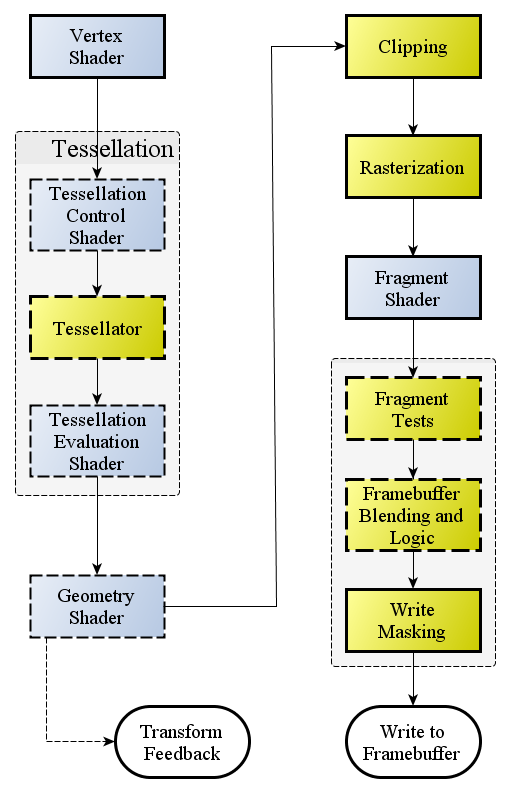
\includegraphics[width=0.5\linewidth]{graphics/RenderingPipeline.png}
    \captionof{figure}[OpenGL]{Diagram of the Rendering Pipeline. The blue boxes are programmable shader stages. \cite{OpenGLPipeline}}
    \label{fig:opengl}
\end{minipage}


\ac{OpenGL} is a low-level graphics API implemented by the video card vendor via the video driver. 
As such it doesn't offer much abstraction over the actual \ac{GPU}, but instead offers high flexibility and performance.
\ac{OpenGL} 1.0 was released in 1992 and the current version is 4.5.
A critical element when developing \ac{OpenGL} applications is, that not all video drivers implement the newest \ac{OpenGL} standards.

As a result, one has to decide which \ac{OpenGL} version to program against, trading between modernity and platform support.
For Romeo, it was decided to support \ac{OpenGL} 3.3 as the lowest bound, as it is sufficiently available, while still having most of the modern features.
The features include instance rendering, vertex arrays and modern \ac{GLSL} shader.

In figure \ref{fig:opengl} you can see the basic architecture of an OpenGL program pipeline.
As the description states, the blue boxes are programmable shaders, while the dotted boxes are optional parts of the pipeline.
The yellow boxes describe stages which are not directly accessible. They're part of the OpenGL state, which can be set via OpenGL commands.

So in order to have a functioning OpenGL rendering pipeline one just needs to write a vertex shader and a fragment shader.

\subsection{Reactive}
Reactive is a functional event system designed for event driven programming.
It implements Elm's signal based event system in Julia.
Signals can be transformed via arbitrary functions which in turn create a new signal.
This simple principle leads too a surprisingly simple yet effective way of programming event based applications.

\begin{lstlisting}
a = Input(40) # an integer signal.
b = Input(2) # an integer signal.
c = lift(+, a,b) # creates a new signal with the callback plus. Equal to c = a+b
lift(println, c) # executes println, every time that c is updated. 
push!(a, 20) # updates a, resulting in c being 22
#prints: 22
push!(b, 5) # updates a, resulting in c being 22
#prints: 25
\end{lstlisting}

\subsection{GLFW}
GLFW is a cross platform \ac{OpenGL} context and window creation library written in C.
GLFW allows to register callbacks for a multitude of events like keyboard, mouse and window events.
This, together with a wrapper library for Julia makes GLFW perfect for doing the window creation.
In addition, GLFW exposes low level features like the operating systems context handle.
This can be used for creating advanced contexts that share memory with another context.
Romeo doesn't use this feature yet, but it makes GLFW a future proof choice.


\section{Implementation}


\vspace{1em}
\begin{minipage}{\linewidth}
    \centering
    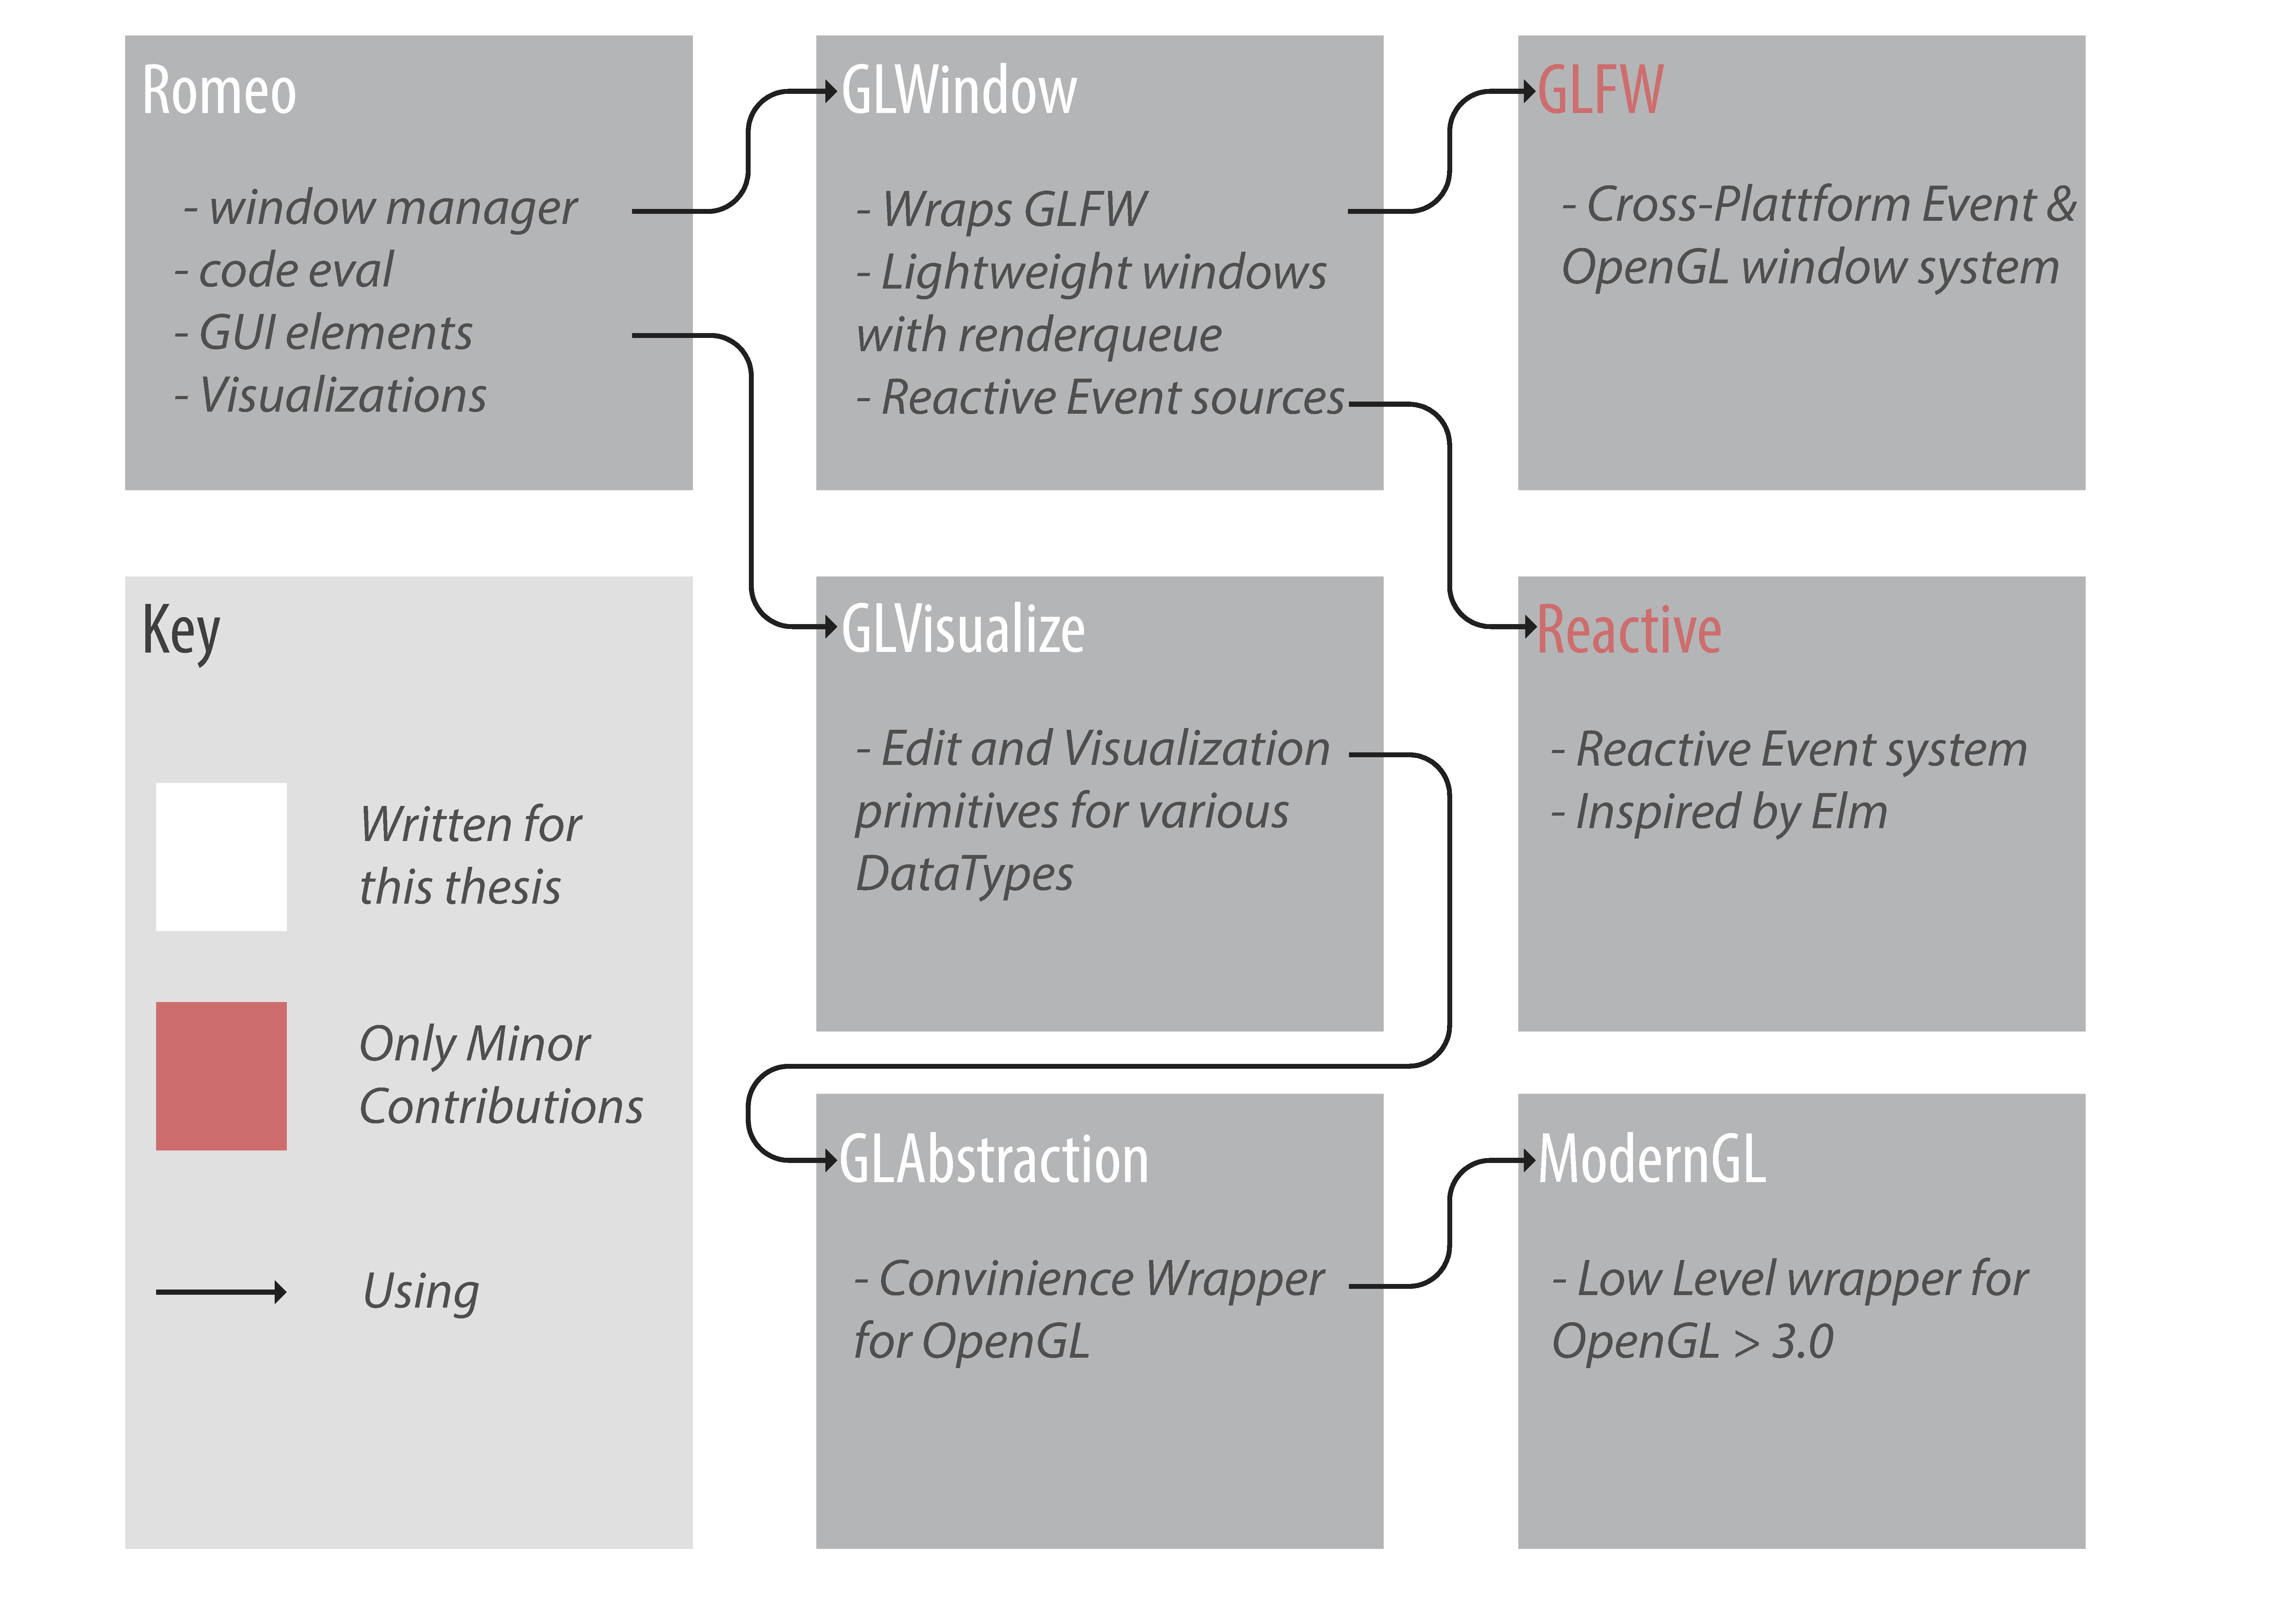
\includegraphics[width=0.9\linewidth]{graphics/architecture.pdf}
    \captionof{figure}[Architecture]{Main modules used in Romeo and their relation (simplified)}
    \label{fig:architecture} 
\end{minipage}


This chapter is about the implementation of Romeo.
The Romeo package itself is small and just defines the high-level functionality of the editor.
This includes window layout and connecting all the different event sources to create the wanted behavior.
To do this, Romeo relies on a multitude of packages, which step for step abstract away the underlying low-level code that is used to do the window creation and rendering.
GLVisualize is the main package offering the rendering functionality and the editor widgets like text fields and sliders.
For rendering GLVisualize relies on GLAbstraction, which defines a high-level interface to \ac{OpenGL}.
\ac{OpenGL} function loading is done by ModernGL, which keeps all the function and Enums definitions from \ac{OpenGL} with version higher than 3.0.
The event management is handled by Reactive.

\subsection{Reactive}

The event system was challenging to integrate for several reasons.
First of all Reactive is a functional event system, while \ac{OpenGL} relies heavily on global states, which are two perpendicular concepts.
Also, it doesn't allow to rearrange the event tree. In other words if you have two signal branches, there is no way to fuse them together.
Finally, it doesn't reuse memory for signals. This means, if you have a signal for a large array every lift operation will allocate new memory for the array.
Working around these shortcomings reduced the ease of use of the overall API.
It has lead to two design choices which are sub optimal.
First, the event system is decoupled from the render loop, to set the global \ac{OpenGL} states appropriately.
This means, that the structure is as follows:
\begin{lstlisting}
#instead of:
a = Input(data)
b = lift(visualize, a)
c = lift(render_opengl, b)
# it is now:
while window.open
	render(b.value)
end
\end{lstlisting}
The sub optimal performance of Reactive for large data has let to the following design:
\begin{lstlisting}
# instead of
a = Input(large_array)
b = lift(some_computation, a, some_timed_signal)
c = lift(visualize, b)
# it is now:
a = visualize(large_array)
lift(some_timed_signal) do time
	b = some_computation(large_array, time)
	update!(a, b) # write directly to the \ac{GPU} object
end
\end{lstlisting}

\subsection{ModernGL}
\ac{OpenGL} is implemented by the video card vendor and is shipped via the video driver, which comes in the form of a C-Library.
The challenge is, to load the function pointer system and vendor independently. Also one further complication is, that depending on the platform, function pointer are only available after an \ac{OpenGL} context was created and may only be valid for this context. \cite{wgl}
This problem is solved, by initializing a function pointer cache with null and as soon as the function is called the first time the real pointer gets loaded. This is suboptimal, as the pointer cannot be inlined and has to be checked for null.
In the newest version of Julia, this can be implemented even more efficiently with staged functions. Staged functions can be thought of as a runtime macro.
At the first call of the function code can be generated, which then will get compiled in time and replaces the function definition. 
This makes the an \ac{OpenGL} function call nearly twice as fast.
Like this, even C can be outperformed in terms of speed, as C doesn't have just in time compilation capabilities, so the function pointers can not be inlined like this. [benchmark pending, probably better in discussion though?]


\subsection{GLAbstraction}
GLAbstraction is the abstraction layer over ModernGL.
It wraps \ac{OpenGL} primitives like Buffers and Textures in Julia objects and hooks them up to Julia's garbage collector.
Additionally, it implements convenient functions to load shader code and it makes it easy to feed the shader with the correct data types.
Besides suplying an abstraction layer over \ac{OpenGL}, it also offers the linear algebra needed for the various 3D transformation and camera code.
Building up on that, it defines a signal based perspective and orthographic camera type.


\subsection{GLWindow}
GLWindow is a lightweight wrapper around GLFW. GLFW is a C-Library, that offers cross-platform \ac{OpenGL} window and context creation and event handling.
GLWindows is the abstraction layer, that builds upon a Julia wrapper of GLFW.
It mainly offers a screen type, which contains signals for all the different GLFW events (Mouse, Keyboard, etc...). 
It also offers a hierarchical structure for nesting screens in each other. 
All the screen areas are signals, which resize the screen area when they change. Like this, you can dynamically have the screen sizes depend on each other and react to resizing the window.



\subsection{GLVisualize}
GLVisualize implements the main functionality of this library.
It offers rendering of different primitives. GLVisiualize is designed with two intentions in mind: supplying a very simple interface consisting of just two functions and transport the data with as little conversions and copies to the GPU.
This allows to manipulate the data directly on the GPU, which is the fastest way to update dynamic data.
The interface to create visualizations is very simple and only consists of two functions:
\begin{lstlisting}
visualization 		  = visualize(data::T, style=Style{:default}; parameters...)
visualization, signal = edit(     data::T, style=Style{:default}; parameters...)
\end{lstlisting}

With this, the following data can be visualized:
\begin{itemize}
	\item Text (Vector of Glyphs)
	\item Height fields with different primitives (Matrix of height values)
	\item 3D bar plots (Matrix of height values)
	\item Images (Matrix of color values)
	\item Videos (Vector of Images)
	\item Volumes (3D Array of intensities)
	\item Particles (Vector of Points)
	\item Vector Fields (3D array of directional Vectors)
	\item Colors (Single Color values)
\end{itemize}

These can be integrated into the same scene. For all of these, it is possible to change their values interactively.
The edit function is making it easier to edit the values of the data.
It calls the visualize function to render the data type and then registers appropriate events to update the data.
Take a look at the text edit function. 
It first uploads the text to video memory and sets up the functionality to visualize it, and than updates the text data on the GPU according to the cursor position and keyboard input.

Up to now, there is only an edit function available for text fields, colors, numbers, vectors and matrices.


\subsubsection{Romeo}
So far Romeo just consists of one file with 500 lines of code. It just defines some simple text field, a search field, and a visualize and edit window.
The texts gets evaluated as Julia code as soon as it changes. Like this, the text field acts like a very simple \ac{REPL}.
Via the search field, you can execute simple Julia statements and the results will be displayed in the visualize window, while all parameters can be edited via the edit window.
This means, if you type in a simple variable, the variable will be visualized. But you can also search and transform a variable via simple Julia terms.